\documentclass[12pt]{article}

\usepackage{graphicx}

\title{COSC 528: Project 2}
\author{Ian Lumsden}

\begin{document}
	\pagenumbering{gobble}
	\maketitle
	\newpage
	\pagenumbering{arabic}
	
	\section{Objective}
	The goal of this project was to categorize UT and its peers using the provided data. In the first part of the project, dimensionality reduction through Principal Component Analysis (PCA) was performed to simplify the data and produce better results during training. In the second part of the project, a K-Means Clustering algorithm was applied to the data (first the original, then the reduced) to determine the other universities in the same grouping as UT. Finally, the second part was repeated using an Expectation-Maximation (EM) algorithm.
	
	\section{Preprocessing}
	The data for this project was provided in several different forms. My implementation is based on "UT-peers.csv". This file consists of 66 feature columns and 187 rows. However, only about 50 of the rows contained data. The remainder were discarded.
	\paragraph{}
	There was a lot of unneeded or missing data in this dataset. To begin cleaning the data, the first, second, third, and fifth columns were dropped, as they contained either unneeded data or invariant data. Next, all discrete data was converted to integers so that it could be used in the models. Then, the financial data columns were altered to remove all dollar signs and commas from the numeric values. Finally, all NaN values were replaced with the mean of their column, and all values were replaced with their corresponding Z-scores.
	
	\section{Principal Component Analysis (PCA)}
	Because this dataset was so large, it was useful to reduce the dimensionality (i.e. number of features) to a more manageable number. This was done using Principal Component Analysis.
	\paragraph{}
	To begin, the preprocessed data, $X$, was factored using singular value decomposition (SVD). This process converts the data into the following
	\begin{equation}
		X = U \Sigma V^T,
	\end{equation}
	where $U$ is an $m x m$ unitary matrix, $\Sigma$ is a diagonal $m x n$ matrix of eigenvalues, and $V$ is a $n x n$ unitary matrix of eigenvectors. The diagonal values of $\Sigma^2$ represent the variance that each principal component covers. By dividing by the sum of variances, the percentage of variance that each primary component covers was obtained. These percentages were plotted against the number of the principal component, as shown in Fig. \ref{Scree}.
	\begin{figure}
		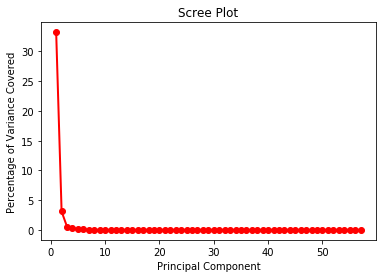
\includegraphics[width=\linewidth]{Pictures/scree.png}
		\caption{Scree Graph for SVD}
		\label{Scree}
	\end{figure}
    \paragraph{}
    From Fig. \ref{Scree}, it is clear that the first two principal components cover most of the data's variance. Using this information, the PCA was performed to produce a two-dimensional reduced dataset. The equations for PCA are as follows
    \begin{equation}
    	W = XV\prime = U\prime S\prime,
    \end{equation}
    where X is the initial dataset, the prime symbol indicates that a matrix has been reduced to its first two columns, and W is the final reduced dataset.
    \paragraph{} 
    After implementing this equation using numpy, a graph (Fig. \ref{PCA}) was made of the two principal components, with one on each axis. For the sake of clarity, the university names were left off of this graph. They can be enabled from the code by setting the "annotate" parameter of "plot\_2PC" to True.
    \begin{figure}
    	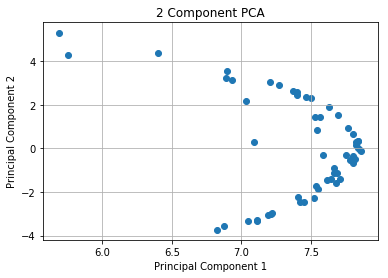
\includegraphics[width=\linewidth]{Pictures/pca.png}
    	\caption{Relationship between the two primary components}
    	\label{PCA}
    \end{figure}

    \section{K-Means Clustering}
    The primary algorithm for this project was K-Means clustering. It is a form of semi-supervised or unsupervised learning that separates data into different categories, or clusters.
    \paragraph{} 
    K-Means clustering is implemented as an iterative model. To begin, $k$ initial "centroids" are chosen at random such that they remain within the bounds of the data. Then, during each iteration, each data row is placed inside the same cluster as its nearest centroid. Once all the data has been sorted into clusters, the centroids are recalculated such that their features are the means of the features of cluster's data. Algebraically, this is represented as
    \begin{equation}
    	m_i^{t+1} = \frac{1}{|S_i^{(t)}|}\sum_{x_j \in S_i^{(t)}}x_j,
    \end{equation}
    where $i$ represents the current cluster, $m$ is a centroid, $S$ is the set of data points in a cluster, and $t$ indicates that a value is current. This algorithm is repeated until the mean-squared Euclidean distance between the old centroids and the new centroids is negilible.
    \paragraph{}
    After implementing the algorithm, it was applied on the original data for various values of $k$, and the Dunn Index was calculated for each repetition. The Dunn Index is simply the ratio of the minimum intercluster distance and the maximum intracluster distance. This data was plotted to determine the best value of $k$ and is shown in Fig. \ref{Dunn}. Based on this graph, it was clear that the best value for $k$ was 2. Using this information, the algorithm was applied with $k = 2$. The resulting data was then used to determine the universities in the same cluster as UT, which can be found in Appendix A. The same process was applied to the data produced by PCA. The Dunn Indices graph for PCA (Fig. \ref{DunnPCA}) showed that the best value for $k$ was also 2. Additionally, the PCA data was replotted in multiple colors to show the clusters (Fig. \ref{PCACluster}). The universities in the same cluster can be found in Appendix B.
    \begin{figure}
    	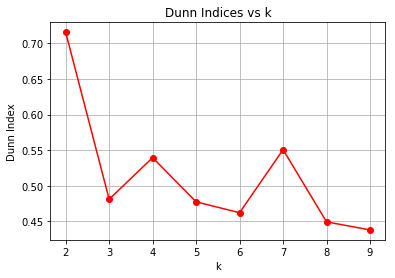
\includegraphics[width=\linewidth]{Pictures/Dunn.png}
    	\caption{Dunn Indices vs k for the Original Data}
    	\label{Dunn}
    \end{figure}
    \begin{figure}
	    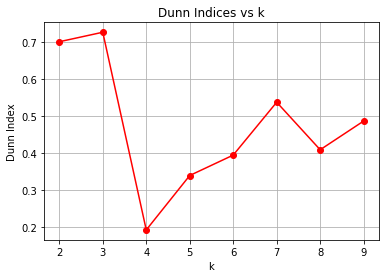
\includegraphics[width=\linewidth]{Pictures/DunnPCA.png}
	    \caption{Dunn Indices vs k for the PCA Data}
	    \label{DunnPCA}
    \end{figure}
    \begin{figure}
    	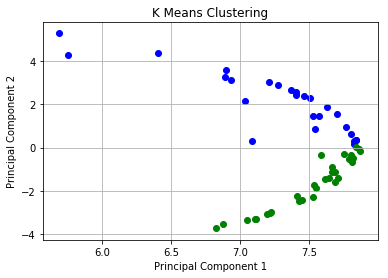
\includegraphics[width=\linewidth]{Pictures/PCACluster.png}
    	\caption{PCA data colored by cluster}
    	\label{PCACluster}
    \end{figure}
    
    \section{Expectation-Maximization Algorithm}
    The final part of this project was implementing the EM algorithm. This algorithm is very similar to K-Means Clustering, but, instead of clustering the data based on hard values, it clusters the data as Gaussian distributions. The algorithm starts by randomly choosing initial mean and standard deviation values for the Gaussian clusters. Like K-Means, EM is an iterative algorithm that consists of two steps. In the first step, the data is assigned the cluster label corresponding with the Gaussian distribution that the data is most likely to be part of. Then, in the second step, the Gaussian parameters (mean and standard deviation) are updated for each cluster. The new means are then compared with the old means. If the Euclidean distance between the two sets is negligible, the algorithm ends.
    \paragraph{}
    After implementing this algorithm, the same procedure that was applied to the original and PCA data for K-Means was applied to the EM algorithm using only the PCA data. As Fig. \ref{DunEM} shows, a $k$ of 2 was best for this EM algorithm. The model was run again to produce the a graph of the clustering of the PCA data and the list of universities that share a cluster with UT. However, as Fig. \ref{EM} shows, this algorithm did not perform well. It is very likely that there was a bug that I was not able to catch that lead to the flat graph and lack of data separation.
    \begin{figure}
    	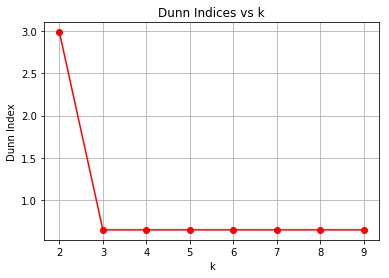
\includegraphics[width=\linewidth]{Pictures/DunEM.png}
    	\caption{Dunn Indecies vs k for the EM Algorithm}
    	\label{DunEM}
    \end{figure}
    \begin{figure}
    	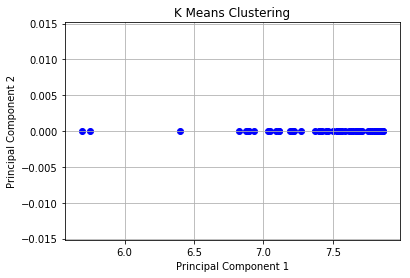
\includegraphics[width=\linewidth]{Pictures/EM.png}
    	\caption{PCA data colored by cluster based on EM}
    	\label{EM}
    \end{figure}

    \newpage
    \section{Conclusions}
    This project demonstrated the use of Principal Component Analysis, K-Means clustering, and the EM algorithm. K-means clustering produced some interesting results, as the PCA data was expected to produce different results that the original data. However, despite the similarity in data, PCA is still more useful since it is easily visualizable in the form of a graph. For the EM algorithm, more work needed to be done to address bugs in the code that resulted in erroneous data. One thing that would likely improve results is the development of a separate graphing algorithm for both the Dunn Indices and the final clustered data. Instead, I used the same functions as I did for K-Means, which likely resulted in some errors.
	
	\section{Code}
	The code is broken down into the following files:
	\begin{enumerate}
		\item \textbf{DataPrep.py}: Code for cleaning the data
		\item \textbf{PCA.py}: Code for performing PCA and plotting associated data
		\item \textbf{KMeans.py}: Code for performing K-Means Clustering on the data and visualizing the results
		\item \textbf{EM.py}: Code for performing the EM algorithm.
		\item \textbf{Driver.ipynb}: Jupyter notebook for controlling the flow of the project.
	\end{enumerate}

    \newpage

    \section{Appendix A}
    \begin{enumerate}
    	\item Univ. of Georgia
    	\item Rutgers Univ.
    	\item Auburn Univ.
    	\item Iowa State Univ.
    	\item NC State Univ.
    	\item Pennsylvania State Univ.
    	\item Ohio State Univ.
    	\item Univ. of Florida
    	\item Univ. of Illinois
    	\item Univ. of California - Los Angeles
    	\item Univ. of California - Santa Barbara
    	\item Univ. of Maryland
    	\item Univ. of Washington
    	\item Louisiana State Univ.
    	\item Virginia Tech
    	\item Univ. of Kentucky
    	\item Mississippi State Univ.
    	\item Univ. of Missouri
    	\item Univ. of Alabama
    	\item Univ. of Mississippi
    	\item Univ. of South Carolina
    	\item Florida State Univ.
    	\item Colorado State
    	\item Arizona State
    	\item Univ. of Massachusetts
    	\item UC-San Diego
    	\item Iowa
    	\item Buffalo
    	\item Arizona
    \end{enumerate}

    \section{Appendix B}
    \begin{enumerate}
    	\item Rutgers Univ.
    	\item Iowa State Univ.
    	\item Pennsylvania State Univ.
    	\item Univ. of California - Davis
    	\item Ohio State Univ.
    	\item Univ. of Florida
    	\item Univ. of Illinois
    	\item Univ. of California - Los Angeles
    	\item Univ. of California - Santa Barbara
    	\item Univ. of Maryland
    	\item Univ. of Washington
    	\item Louisiana State Univ.
    	\item Virginia Tech
    	\item Univ. of Kentucky
    	\item Univ. of Missouri
    	\item Univ. of Mississippi
       	\item Univ. of South Carolina
    	\item Florida State Univ.
    	\item Colorado State
    	\item Arizona State
    	\item Univ. of Massachusetts
    	\item SUNY - Stony Brook
    	\item UC-Irvine
    	\item UC-San Diego
    	\item Connecticut
    	\item Iowa
    	\item Buffalo
    	\item Utah
    	\item UC-Riverside
    	\item Arizona
    \end{enumerate}
	
\end{document}